We tested that explanation rather than asserting it. Over $250$ instances in
each stratum we recorded, for every certified arrowhead, whether the frozen
block $Z_{ij}$ contained every parent of $i$ and of $j$, and whether the
arrowhead was wrong. Table~\ref{tab:diag} reports the result. Note that these
are per-\emph{arrowhead} rates, whereas Table~\ref{tab:main} reports
per-\emph{run} rates.

\begin{table}[t]
\centering
\caption{Wrong-arrowhead rate by whether the frozen conditioning block
contained every parent of both endpoints, $250$ instances per stratum, Wilson
$95\%$ intervals. Rates are per certified arrowhead.}\label{tab:diag}
\footnotesize
\begin{tabular}{@{}llccc@{}}
\toprule
stratum & $Z_{ij}$ & arrowheads & wrong & rate \\
\midrule
premise holds & complete   & $486$ & $2$  & $0.004$ \tiny{[.001,.015]} \\
premise holds & incomplete & $224$ & $3$  & $0.013$ \tiny{[.005,.039]} \\
premise fails & complete   & $465$ & $3$  & $0.007$ \tiny{[.002,.019]} \\
premise fails & incomplete & $447$ & $22$ & $0.049$ \tiny{[.033,.073]} \\
\bottomrule
\end{tabular}
\end{table}

Both halves of the explanation hold. Incompleteness is more common where the
premise fails---$49.0\%$ of certified arrowheads against $31.5\%$ where it
holds (Fisher $p = 1.4\times10^{-12}$)---which is the certification-order
effect. And incompleteness is where the errors are: on the failing stratum the
wrong-arrowhead rate is $0.049$ with an incomplete block against $0.007$ with
a complete one, a factor of $7.6$ (Fisher $p = 5.5\times10^{-5}$), and $22$ of
the $25$ wrong arrowheads occur on pairs with an incomplete block. These are
per-arrowhead rates, not the quantity $\alpha_D$ bounds: $\alpha_D$ is a
whole-run, family-wise budget summed over all $d(d-1)$ direction nulls
(Section~\ref{sec:algo-desc}), so the two are not on a common scale and the
per-arrowhead rate being numerically smaller than $\alpha_D$ is not itself a
statement that any budget is respected. What the stratification does support
is the qualitative claim already made: the errors are not spread evenly but
concentrated on the incomplete-block cells, which is where
Theorem~\ref{thm:main}'s direction premise is violated.

\begin{figure}[t]
\centering
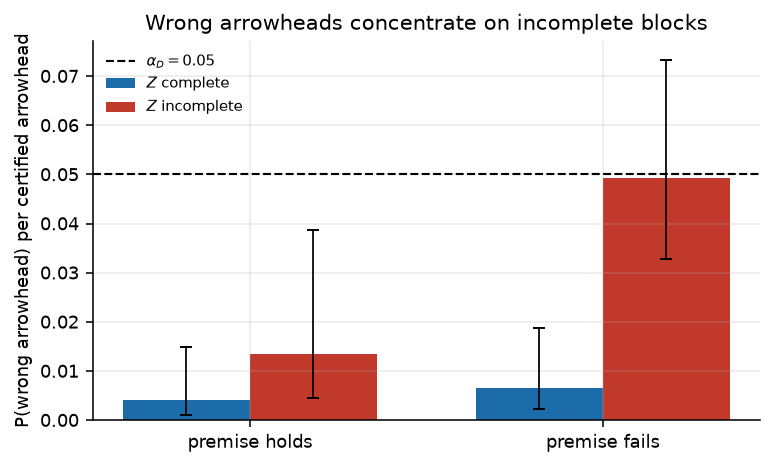
\includegraphics[width=0.72\textwidth]{figs/exp11_block_completeness.png}
\caption{Wrong-arrowhead rate by conditioning-block completeness, with Wilson
$95\%$ intervals. The dashed line marks $\alpha_D$'s numerical value for
scale only: $\alpha_D$ bounds the whole-run, family-wise probability of any
wrong arrowhead over all $d(d-1)$ direction nulls, not the per-arrowhead rate
plotted here, so a bar falling below the line is not a budget statement. The
exceedance in Table~\ref{tab:main} lives entirely in the incomplete-block bar
on the premise-failing stratum.}\label{fig:exp11}
\end{figure}

Figure~\ref{fig:exp11} plots the four cells at the same numerical scale as
$\alpha_D$, without claiming the two are the same quantity.

The exceedance in Table~\ref{tab:main} is therefore not a failure of
Proposition~\ref{prop:direction} or of its implementation. It is the
misspecification gap of Remark~\ref{rem:misspec} being opened by a specific,
identifiable mechanism, and it is reached through the algorithm's own
scheduling rather than through anything intrinsic to the direction null.
